%% bare_jrnl_comsoc.tex
%% V1.4b
%% 2015/08/26
%% by Michael Shell
%% see http://www.michaelshell.org/
%% for current contact information.




% *** Authors should verify (and, if needed, correct) their LaTeX system  ***
% *** with the testflow diagnostic prior to trusting their LaTeX platform ***
% *** with production work. The IEEE's font choices and paper sizes can   ***
% *** trigger bugs that do not appear when using other class files.       ***
% The testflow support page is at:
% http://www.michaelshell.org/tex/testflow/


\documentclass[journal,comsoc]{IEEEtran}
%
% If IEEEtran.cls has not been installed into the LaTeX system files,
% manually specify the path to it like:
% \documentclass[journal,comsoc]{../sty/IEEEtran}

\newcommand\notsotiny{\@setfontsize\notsotiny{6}{7}}
\usepackage[T1]{fontenc}% optional T1 font encoding

% Some very useful LaTeX packages include:
% (uncomment the ones you want to load)

\usepackage{amsmath,amssymb,amsfonts}
% \usepackage{amsfonts} % to load math symbols
\usepackage{commath} % For defining functions
\usepackage{mdwmath}
% \usepackage{showframe}
% \usepackage{mdwtab}
% \usepackage{minipage}
% \usepackage[keeplastbox]{flushend}
\usepackage{graphicx}
% \usepackage{etoolbox}
\usepackage{color}
% \usepackage{placeins}
% \usepackage{subfigure}
\usepackage{subfig}
\usepackage{caption}
\usepackage[nolist]{acronym}
% \usepackage{hyperref}
% % The following is done to hide ugly color boxes around the links
\usepackage[table]{xcolor}
% \hypersetup{
% colorlinks,
% linkcolor={black},
% citecolor={black},
% urlcolor={black}
% }
\usepackage{booktabs}
\usepackage{float}
\usepackage{newtxtext,newtxmath}
% \usepackage{geometry} % just not to bother with the table width
% \usepackage{standalone}
% \usepackage{filecontents}
\usepackage{tabularx,colortbl}
\usepackage{pgfplots}
\usepackage{standalone}
\usepackage{tikz}
\tikzset{
font={\fontsize{10pt}{10}\selectfont}}
\usepackage{tikzscale} % Scale the figure not the font
\pgfplotsset{compat=newest}
\usetikzlibrary{patterns}
%% the following commands are sometimes needed
\usepackage{grffile}
\usepackage{mathtools}
\usepackage[separate-uncertainty = true,
multi-part-units = repeat]{siunitx}
\sisetup{per=slash, load=abbr, output-complex-root = j, complex-root-position = before-number}

% *** CITATION PACKAGES ***
%
% \usepackage{cite}
\usepackage[noadjust]{cite}


% *** GRAPHICS RELATED PACKAGES ***
%
% \usepackage{graphicx}
% declare the path(s) where your graphic files are
\graphicspath{{Figures/}}
%
% Personal definitions
\renewcommand{\v}[1]{\mathbf{#1}} % vectors
\newcommand{\ti}[1]{\tilde{#1}} % spectral representation
\newcommand{\tnsr}[1]{\underline{\underline{#1}}}
% Operators
\renewcommand{\O}{\omega}  % omega
\newcommand{\E}{\varepsilon}  % epsilon
\renewcommand{\u}{\mu}  % mu
\newcommand{\p}{\rho}  % rho
\newcommand{\vp}{\boldsymbol \p}  % rho
\newcommand{\x}{\times}  % times
\renewcommand{\inf}{\infty}  % infinity
\newcommand{\infint}{\int\limits_{-\inf}^\inf} % integral by R
\renewcommand{\del}{\nabla}  % nabla operator
\renewcommand{\^}{\hat}  % unit vector
\newcommand*\diff{\mathop{}\!\mathrm{d}} % Define differential operator
\newcommand{\e}{\mathrm{e}} % Straight-up exponential
\renewcommand{\j}{{j}\mkern1mu} % Straight-up exponential
\newcommand{\iu}{\mathrm{i}\mkern1mu}


% *** Do not adjust lengths that control margins, column widths, etc. ***
% *** Do not use packages that alter fonts (such as pslatex).         ***


% correct bad hyphenation here
\hyphenation{op-tical net-works semi-conduc-tor}


\begin{document}
%
\title{Support Vector Machine to Predict Type 2 Diabetes using Oral Glucose Tolerance Test}
%
% use \thanks{} to gain access to the first footnote area
% a separate \thanks must be used for each paragraph as LaTeX2e's \thanks
% was not built to handle multiple paragraphs
%

\author{Hasan~T.~Abbas,~
Lejla~Alic,~
Madhav~Erraguntla,~
Muhammad Abdul-Ghani,~
Jim~X.~Ji,~\IEEEmembership{Senior Member,~IEEE,}
Qammer~H.~Abbasi,~\IEEEmembership{Senior Member,~IEEE,}
and~Marwa~Qaraqe,~\IEEEmembership{Member,~IEEE}% <-this % stops a space
\thanks{H. T. Abbas and J. X. Ji are with the Department
of Electrical and Computer Engineering, Texas A\&M University at Qatar, Doha 23874 Qatar;  {hasan.abbas;jim.ji}@qatar.tamu.edu}% <-this % stops a space
\thanks{L. Alic was with the Department
of Electrical and Computer Engineering, Texas A\&M University at Qatar, Doha 23874 Qatar; lejlaresearch@gmail.com}% <-this % stops a space
\thanks{M. Erraguntla is with the Department of Industrial and Systems Engineering, Texas A\&M University, College Station, TX 77843; merraguntla@tamu.edu}% <-this % stops a space
\thanks{M. Abdul-Ghani is with the UT Health, San Antonio, TX 78229; abdulghani@uthscsa.edu}% <-this %
\thanks{Q. H. Abbasi is with the School of Engineering, University of Glasgow, UK; qammer.abbasi@glasgow.ac.uk}% <-this %
\thanks{M. Qaraqe is with the College of Science and Engineering, Hamad Bin Khalifa University Doha, Qatar; mqaraqe@hbku.edu.qa}% <-this % stops a space stops a space
\thanks{Manuscript received April 19, 2005; revised August 26, 2015.}}

% note the % following the last \IEEEmembership and also \thanks -
% these prevent an unwanted space from occurring between the last author name
% and the end of the author line. i.e., if you had this:
%
% \author{....lastname \thanks{...} \thanks{...} }
%                     ^------------^------------^----Do not want these spaces!
%
% a space would be appended to the last name and could cause every name on that
% line to be shifted left slightly. This is one of those "LaTeX things". For
% instance, "\textbf{A} \textbf{B}" will typeset as "A B" not "AB". To get
% "AB" then you have to do: "\textbf{A}\textbf{B}"
% \thanks is no different in this regard, so shield the last } of each \thanks
% that ends a line with a % and do not let a space in before the next \thanks.
% Spaces after \IEEEmembership other than the last one are OK (and needed) as
% you are supposed to have spaces between the names. For what it is worth,
% this is a minor point as most people would not even notice if the said evil
% space somehow managed to creep in.



% The paper headers
\markboth{Journal of \LaTeX\ Class Files,~Vol.~14, No.~8, August~2015}%
{Shell \MakeLowercase{\textit{et al.}}: Bare Demo of IEEEtran.cls for IEEE Communications Society Journals}
% The only time the second header will appear is for the odd numbered pages
% after the title page when using the twoside option.
%
% *** Note that you probably will NOT want to include the author's ***
% *** name in the headers of peer review papers.                   ***
% You can use \ifCLASSOPTIONpeerreview for conditional compilation here if
% you desire.




% If you want to put a publisher's ID mark on the page you can do it like
% this:
%\IEEEpubid{0000--0000/00\$00.00~\copyright~2015 IEEE}
% Remember, if you use this you must call \IEEEpubidadjcol in the second
% column for its text to clear the IEEEpubid mark.



% use for special paper notices
%\IEEEspecialpapernotice{(Invited Paper)}




% make the title area
\maketitle

% As a general rule, do not put math, special symbols or citations
% in the abstract or keywords.
\begin{abstract}
  Diabetes is a large healthcare burden worldwide. There is substantial evidence that lifestyle modifications and drug intervention can prevent diabetes, therefore, an early identification of high risk individuals is important to design targeted prevention strategies. In this paper, we present an automatic tool that uses machine learning techniques to predict development of type 2 diabetes mellitus (T2DM). Data generated from an oral glucose tolerance test (OGTT) was used to develop a predictive model based on the support vector machine (SVM). We trained and validated the models using the OGTT and demographic data of 1,496 healthy individuals collected during the San Antonio Heart Study. This study collected plasma glucose and insulin concentrations before glucose intake and at three time-points thereafter (30, 60, and 120 minutes). Furthermore, personal information as age, ethnicity and body-mass index was also a part of the dataset. Using 11 blood measurements, we have deduced 61 features, which are then assign a rank and the top ten features are shortlisted using Minimum Redundancy Maximum Relevance feature selection algorithm. All possible combinations of the 10 best ranked features were used to generate the SVM based prediction models.  This research shows that an individual's abnormal plasma glucose levels, and the information derived therefrom have the strongest predictive performance. Significantly, the insulin and demographic features do not provide additional performance improvement for diabetes prediction. The results of this work identify the parsimonious clinical data needed to be collected for an efficient prediction of T2DM. Our approach shows an average accuracy of 96.81\% and a specificity of 80.45\% obtained on a holdout set.
\end{abstract}


%
% Note that keywords are not normally used for peer-review papers.
\begin{IEEEkeywords}
  Type 2 Diabetes prediction, machine learning, disease risk assessment, San Antonio heart study.
\end{IEEEkeywords}
%
% For peer review papers, you can put extra information on the cover
% page as needed:
% \ifCLASSOPTIONpeerreview
% \begin{center} \bfseries EDICS Category: 3-BBND \end{center}
% \fi
%
% For peerreview papers, this IEEEtran command inserts a page break and
% creates the second title. It will be ignored for other modes.
\IEEEpeerreviewmaketitle
%
%
%
\section{Introduction}
% The very first letter is a 2 line initial drop letter followed
% by the rest of the first word in caps.
%
% form to use if the first word consists of a single letter:
% \IEEEPARstart{A}{demo} file is ....
%
% form to use if you need the single drop letter followed by
% normal text (unknown if ever used by the IEEE):
% \IEEEPARstart{A}{}demo file is ....
%
% Some journals put the first two words in caps:
% \IEEEP\citeARstart{T}{his demo} file is ....
%
% Here we have the typical use of a "T" for an initial drop letter
% and "HIS" in caps to complete the first word.
\IEEEPARstart{T}{he} global incidence of diabetes was estimated at \num{422} million in the year \num{2014} and its prevalence among the adult population increased from \SI{4.7}{\percent} in \num{1980} to \SI{8.5}{\percent} in \num{2014} \cite{mathers_projections_2006}. In \num{2015} alone, an estimated \num{1.6} million deaths worldwide were attributed to diabetes. In addition to the high mortality rate, an individual with diabetes is at a greater risk of developing cardiovascular diseases, visual impairment and limb amputations, as compared to a non-diabetic individual. Due to the substantial socio-economic burdens that are associated with diabetes, its early detection, prevention, and management has become a worldwide top-level health concern. There is experimental evidence that the development of diabetes can be delayed or even prevented provided an individual undertakes a lifestyle change that includes diet management, adopting exercise, and adhering to a pharmacological treatment \cite{tuomilehto2001prevention}. The early identification of high risk individuals of diabetes is therefore, essential for targeted prevention strategies \cite{diabetes2015long}.

Even though the number of clinical studies aimed at diagnosing diabetes have been growing in the last two decades, studies predicting the risk of developing diabetes are limited. This subject has lately received an increased amount of research interest \cite{noble2011risk}. However, the clinical significance of such predictions largely depend on the type and quality of data collected. There are studies that assign a probability to the future risk of diabetes using socio-demographic characteristics such as age, ethnicity, \ac{bmi} and genealogical information collected through population  \cite{Heikes1040, Glumer727}. Due to the unreliable data collection, such techniques can be misleading. The collection of blood samples, on the other hand, provides more reliable data and is a first step towards the disease prognosis with a deeper clinical insight \cite{HELIOVAARA1993181}. \ac{ogtt} is commonly used to screen diabetes \cite{expert-committee} and to provide a critical understanding of its future evolution \cite{stumvoll_use_2000}. In an \ac{ogtt}, the plasma glucose and insulin levels are measured at regular intervals in a 2-hr period after orally administering a standard dose of glucose \cite{stumvoll_use_2000}. The glucose tolerance and insulin resistance are two of the most significant parameters deduced from the \ac{ogtt} that are widely regarded as the major factors in the development of \ac{t2dm}.

A precursory stage of diabetes, commonly referred to as prediabetes, exists before overt \ac{t2dm}, and is described by an \ac{igt}. According to the \ac{who} diagnostic criteria, the \ac{igt} is defined as fasting plasma glucose level of \SI[round-mode = off,group-separator = {,}]{> 126}{\milli\gram\per\deci\liter} and a 2-hour plasma glucose level in the range of \SIrange[round-mode = off,group-separator = {,}]{140}{199}{\milli\gram\per\deci\liter}, measured during the \ac{ogtt} \cite{organization_definition_2006}. Although prediabetes is considered as an intermediate stage in the natural progression of \ac{t2dm} \cite{defronzo2011assessment}, it has been reported that only \SI{50}{\percent} of the subjects diagnosed with \ac{igt} developed diabetes within 10 years \cite{shaw_impaired_1999, writing_committee_impaired_2002}. Moreover, long-term population studies have also shown that around \SI{50}{\percent} of the diabetic patients did not exhibit \ac{igt} at any time prior to the diagnosis \cite{abdul-ghani_what_2007}. This suggests that the fasting and 2-hour plasma glucose levels used in and of themselves cannot accurately predict the future development of \ac{t2dm}.

\ac{ml} has been proposed as a viable instrument for diabetes screening. In contrast to traditional diagnostic techniques employing population based statistics, \ac{ml} methods develop models that are trained using large amounts of data. Barakat et al used socio-demographic information, and point of care testing from blood and urine to develop diagnostic models of diabetes \cite{barakat_intelligible_2010}. This approach uses \ac{svm} along with a rule-based explanation to provide a comprehensibility of the results to the clinicians. The plasma glucose levels at baseline and 2-hr were among the features used. Han et al employed an ensemble \ac{svm} and random forest learning approaches to develop a decision making algorithm for the diagnosis of diabetes \cite{han_rule_2015}. However, investigations that are designed to identify individuals at high risk of developing \ac{t2dm} in future are limited. The \ac{sadpm} \cite{stern2002identification} uses a logistic regression supported by physiological parameters such as systolic blood pressure and cholesterol level. The underlying causes of \ac{t2dm} in the form insulin resistance and insulin secretion were studied to develop a prediction model in \cite{abdul-ghani_what_2007}. In another study, multivariate logistic models using the plasma glucose values measured in the \ac{ogtt} were used to predict the future risk of developing \ac{t2dm} \cite{abdul-ghani_two-step_2011,abdul2009fasting}. The predictive power of different biomarkers such as the fasting plasma glucose level, \ac{bmi} and hemoglobin A1C (HbA1c) for \ac{t2dm} onset was assessed in \cite{Ozery-Flato2013}. This study focused on individuals with metabolic syndrome, a complex and serious health condition that greatly increases the risk of \ac{cvd} and diabetes.

The standard \ac{ml} algorithms are designed to yield optimal performance in terms of accuracy over the full dataset. However, medical applications such as disease diagnosis and prediction require a biased decision-making mechanism that favors one of the classes. This approach inherently maximizes the performance of the class that is more relevant in clinic terms. Therefore, the objective in such applications is to design a classifier that improves the accuracy of the class that is clinically more relevant. Additionally, often the amount of data is highly skewed with the clinically relevant class in an outsized minority. There are various roundabout ways to obtain accurate classifier performance in this scenario that include the method of sampling \cite{chawla2002smote} in which the class distribution is artificially balanced by either under sampling the majority class, over-sampling the minority class or both. Furthermore, feature weighting schemes assign distinct costs to training examples \cite{Domingos} in order to introduce a certain bias. Other techniques introduce evaluation metric such as the \ac{gm} \cite{kubat1997addressing}, that concurrently optimizes the positive class accuracy (sensitivity) and the negative class accuracy (specificity) \cite{Tang_SVM}.

We hypothesized that the features extracted from the \ac{ogtt} will be able to predict the future onset of \ac{t2dm}. In this paper, we therefore propose a screening tool that identifies the most relevant features extracted from the \ac{ogtt} data that strongly correlate with the future development of \ac{t2dm}. We then use \ac{svm} to develop a prediction model by utilizing these relevant features estimated from the longitudinal cohort study, the \ac{sahs} \cite{burke_rapid_1999,lorenzo_trend_2006}.
%
\section{Materials and Methods}
%
\subsection{San Antonio Heart Study}
%
The SAHS is a population-based epidemiological study that was conducted to assess the risk factors of diabetes and cardiovascular diseases in healthy population \cite{burke_rapid_1999,lorenzo_trend_2006}. In total, \num[group-minimum-digits=4, group-separator = {,}]{5158} men and non-pregnant women of \ac{ma} and \ac{nhw} residents of San Antonio, Texas participated in the study in two cohorts. The age of the individuals at the time of recruitment was between \num{25} and \num{64} years. As a part of the data collection, the plasma glucose and insulin concentrations were collected during the oral glucose tolerance test at the baseline and after an average follow-up of \num{7.5} years. The \ac{bmi} was also recorded for each individual at the baseline. In this study, we analyzed only the data generated from the second cohort of the \ac{sahs} which comprised \num[group-minimum-digits=4, group-separator = {,}]{1492} subjects from the second cohort of the SAHS.

\ac{t2dm} was diagnosed at the follow-up using the \ac{who} criteria, i.e. fasting glucose level \SI[round-mode = off,group-separator = {,}]{> 126}{\milli\gram\per\deci\liter} or 2-hr glucose level \SI[round-mode = off,group-separator = {,}]{\ge 200}{\milli\gram\per\deci\liter} \cite{organization_definition_2006}. Furthermore, all individuals taking anti-diabetic medications were also classified as having \ac{t2dm}. Individuals that reported by themselves any cardiovascular event such as heart attack, stroke or angina, were labeled as having \ac{cvd} at the follow-up. All other participants without \ac{t2dm} or self-reported \ac{cvd} were labeled as healthy for the case of this study. During the course of the longitudinal study, a total of \num{171} individuals developed \ac{t2dm} with \num{10} individuals also reporting at least one cardiovascular event. The incidence rate of \ac{t2dm} in the second cohort of the \ac{sahs} population was \SI{10.79}{\percent}. Table \ref{tab:patients} shows the population distribution in terms of the four classes. The distribution in terms of the ethnicity shows a more than double \ac{t2dm} prevalence among the \ac{ma} individuals, as compared to the \ac{nhw} population.
%
\begin{table}[!h]
  \centering
  \renewcommand{\arraystretch}{1.3}
  \caption{The classification of the \num[group-minimum-digits=4, group-separator = {,}]{1492} subjects used in this study}
  % \vspace{-4mm}%Put here to reduce too much white space after table
  \centering
  \begin{tabular}{c c c c c}
    \toprule
    & Healthy &  \ac{t2dm} & \ac{cvd} & \ac{t2dm}+\ac{cvd}\\
    \midrule \midrule
    Total & \num[group-minimum-digits=4, group-separator = {,}]{1277} & \num{161} & \num{44} & \num{10}\\
    &\SI{85.56}{\percent} & \SI{10.79}{\percent} & \SI[round-precision=3]{2.95}{\percent} & \SI[round-precision=2]{0.67}{\percent} \\
    \midrule
    \ac{ma} & \num[group-minimum-digits=4, group-separator = {,}]{836} & \num{131} & \num{24} & \num{7}\\
    &\SI{83.77}{\percent} & \SI{13.13}{\percent} & \SI[round-precision=3]{2.40}{\percent} & \SI[round-precision=2]{0.70}{\percent} \\
    \midrule
    \ac{nhw} & \num[group-minimum-digits=4, group-separator = {,}]{441} & \num{30} & \num{20} & \num{3}\\
    &\SI{89.27}{\percent} & \SI{6.07}{\percent} & \SI[round-precision=3]{4.05}{\percent} & \SI[round-precision=2]{0.61}{\percent} \\
    \bottomrule
  \end{tabular}
  \label{tab:patients}
\end{table}
%
\begin{figure*}[t!]
	\centering
	\subfloat[Plasma Glucose]
  {
  \includegraphics[width=.45\textwidth]{boxpl_glucose.tikz}
	\label{fig:glucose}
  }
	\subfloat[Serum Insulin]
  {
  \includegraphics[width=.45\textwidth]{boxpl_Insulin.tikz}
  \label{fig:insulin}
  }
	\caption{Box plots of glucose and insulin levels for healthy and diabetic subjects measured at the baseline \ac{ogtt}.}
  \label{fig:ogtt_mean}
\end{figure*}
% \begin{figure*}[t!]
%   \centering
%   \begin{subfigure}[b]{\columnwidth}        %% or \columnwidth
%     \centering
%     \includegraphics[width=.9\linewidth]{boxpl_glucose.tikz}
%     \label{fig:glucose}
%   \end{subfigure}
%   \hfill
%   \begin{subfigure}[b]{\columnwidth}        %% or \columnwidth
%     \centering
%     \includegraphics[width=.9\linewidth]{boxpl_Insulin.tikz}
%     \label{fig:insulin}
%   \end{subfigure}
%   \caption{Box plots of glucose and insulin levels for healthy and diabetic subjects measured at the baseline \ac{ogtt}.}
%   \label{fig:ogtt_mean}
% \end{figure*}
The data used in this study consists of the plasma glucose and insulin concentrations sampled at baseline, and at \num{30}, \num{60} and \SI{120}{\minute} thereafter. The individuals are labeled at the SAHS follow-up using the current standard of care \cite{burke_rapid_1999}. Figure \ref{fig:ogtt_mean} shows the distributions of the data used in this study.
%
%
\subsection{Machine Learning Framework}
%
In this paper, we implemented \ac{svm} to construct the models for prediction of future \ac{t2dm}. The \ac{svm} develops models from a given training dataset such that it generalizes well to a new dataset and minimizes the empirical risk associated with misclassification of samples in the training set \cite{vapnik_nature_2000,vapnik2015uniform}. A model constructed by the \ac{svm} minimizes the overlap between the classes in the training set by optimizing the separating hyperplane. For problems that may not be amenable to linear separation between the two classes, the \ac{svm} technique is very attractive due to fact that the input feature space can be transformed to a higher dimension space,  and a linear boundary can then be determined. This approach generally provides a better training performance but potentially increases computational complexity excessively with the increase of the dimensionality of the input feature space \cite{friedman2001elements}. Introduction of a kernel alleviates the need to determine the transformation by calculating the inner product between the coordinates of the input feature space instead. In this paper, we used the Gaussian \ac{rbf},  as the kernel. The performance of the \ac{svm} can be optimized by tuning the free parameter of the kernel $\sigma$ and specifying a cost that controls the rigidity of the class margin. This process is normally carried out through a grid search.
%
%
%
%
\subsection{Feature Extraction}
%
We extracted all the features from the \ac{sahs} data acquired at the baseline. The dataset consists of the plasma glucose and insulin concentrations recorded before glucose intake and at three time-points thereafter (\num{30}, \num{60}, and \SI{120}{\minute}). The labels (healthy and diabetes) were generated at the \num{7.5} years follow-up using the current standard of care diagnostics \cite{burke_rapid_1999}. From the glucose and insulin concentrations, we computed the slope and area under the curve between all the possible combinations of a pair of measurements. In addition, we also calculated three empirical markers that describe the relationship between the glucose intake and insulin response. The first is the \ac{igi} \cite{seino1975insulinogenic}, which is a direct measure of the insulin response to glucose. It is calculated as the ratio of the slope of insulin curve to the slope of glucose curve between any two progressive time intervals in the \ac{ogtt}. The second marker, \ac{mi}  $\mathrm M$, evaluates the insulin sensitivity from the \ac{ogtt} using a product of the weighted averages of the glucose and insulin concentrations \cite{Matsuda1462},
%
\begin{equation}
  \mathrm{M} = \frac{10,000}{\sqrt{Glu_0 \times Ins_0 \times \frac{15 Glu_0 + 30 Glu_{30} + 30 Glu_{60} + 30 Glu_{90} + 15 Glu_{120}}{120} \times \frac{15 Ins_0 + 30 Ins_{30} + 30 Ins_{60} + 30 Ins_{90} + 15 Ins_{120}}{120}}},
  \label{eq:mat_idx}
\end{equation}
%
where the subscripts depict the time point of the OGTT. In case when the value at 90 minutes is not available, the average of 60 and 120 minutes is used instead \cite{Matsuda1462}. The third marker, \ac{homair} \cite{matthews1985homeostasis} evaluates the beta-cell function. It is defined as the product of fasting plasma glucose concentration and fasting blood insulin concentration divided by \num{22.5}. These markers have been used to estimate abnormalities in the insulin sensitivity. A total of \num{61} features (illustrated in Fig. 2) are used in this study. The prefix AuC denotes the area under the curve and the slope is denoted by the symbol $\Delta$. The term T\textsubscript{half} represents the linearly interpolated value between any two intervals. The \ac{ogtt} time interval in minutes corresponding to the feature appears in the subscripts.
%
\begin{figure*}[t!]
  \centering
  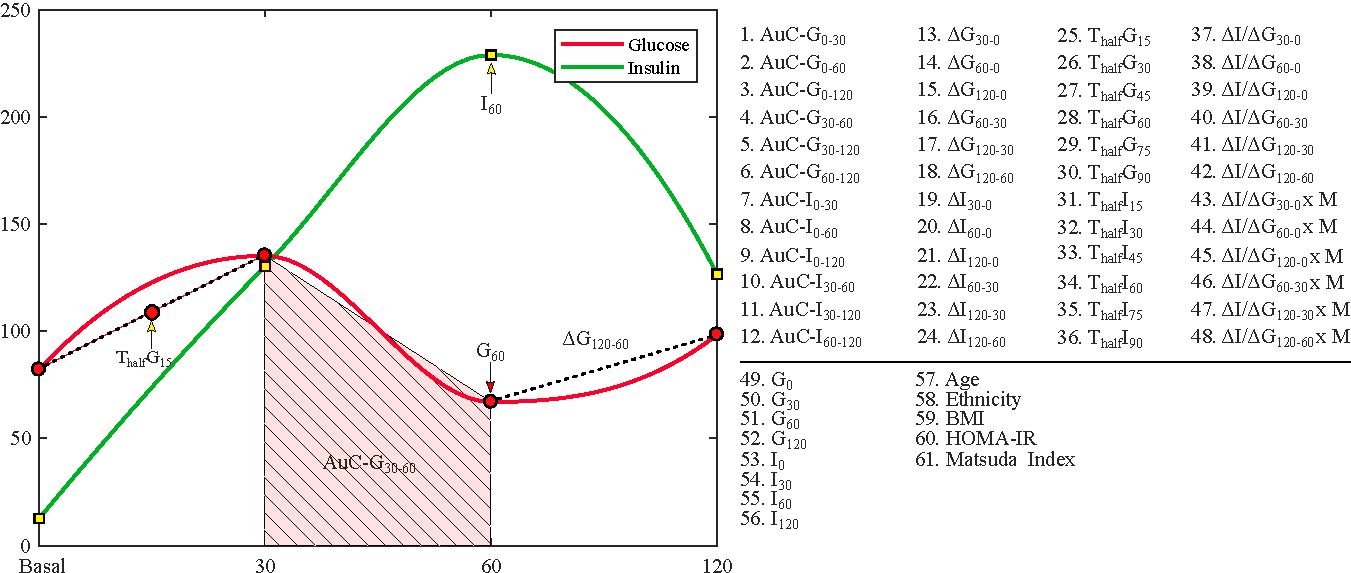
\includegraphics[width=.9\linewidth]{features_define_text.pdf}
  \caption{Illustration of all 61 features extracted from the \ac{sahs} dataset.}
  \label{fig:features}
\end{figure*}
%
%
%
%
\subsection{Feature Selection}
%
Before constructing the \ac{svm} model to predict a future diabetes occurrence, we search for the most effective subset of features in terms of relevance to the classifier output, i.e. incidence of \ac{t2dm} at the follow-up. As a first step, we selected the ten most relevant features from the \num{61} available features using the \ac{mrmr} algorithm \cite{mRMR}, which selects the most relevant features with minimum correlation among them. The \ac{mrmr} algorithm determines the relevance between a feature ($x$ as continuous random variable) and the class label ($y$ as discrete random variable) in terms of the mutual information $\mathcal I$ defined as \cite{ross2014mutual},
%
\begin{equation}
  \mathcal I(x, y) = - \int p_i \ln p_i \diff x - \sum \limits_j p_j\ln p_j + \sum_j \int p_{ij}\ln p_{ij} \diff x,
  \label{eq:MI}
\end{equation}
%
where $p_{i}$, and $p_{j}$ are the probabilities of the random variables $x$ and $y$ taking a particular value $x_i$ and $y_j \in (-1,1) \, \forall j$ respectively. The term $p_{ij}$ denotes the joint probability $P\{x= x_i, y=y_j\}$. The three terms in \eqref{eq:MI} represent the continuous, discrete and joint entropies of the random variables in the respective order. The features that are most relevant to the class label are the ones that maximize $\mathcal I$. A heuristic approach is to keep only one a single feature from a correlated set of features that provides similar relevance information, and discard the remaining features. In order to ensure this, the \ac{mrmr} algorithm minimizes the mutual correlation among the features expressed in terms of redundancy $\mathcal R$,
%
\begin{equation}
  \mathcal R(\mathbb X) = \sum \limits_{x_i, x_j \in \mathbb{X}} \mathcal {I}(x_i, x_j).
  \label{eq:R}
\end{equation}
%
where $\mathcal I$ follows its definition in \eqref{eq:MI}. This procedure yielding maximum $\mathcal I$ with respect to the diabetic class, along with minimal $\mathcal R$, shortlists a set of ten features that are potentially strong predictors of the future development of \ac{t2dm}.
%
%
%
%
\subsection{Classification}
%
We developed a supervised learning scheme using the baseline \ac{sahs} dataset and the labels (healthy, \ac{t2dm}) obtained at the follow-up after an average of \num{7.5} years. In each experiment, we used a kernel-based binary \ac{svm} method to train, test and validate the performance of the diabetes prediction models.  We excluded the \num{44} \ac{cvd} entries as the only way of defining this class was based upon self-reporting and not on quantitative assessment. Furthermore, we also removed all entries with any information missing. That resulted in a total of \num[group-minimum-digits=4, group-separator = {,}]{1492} instances that were used in this study, out of which \num{171} were from the minority class and \num[group-minimum-digits=4, group-separator = {,}]{1321} were majority instances. As shown in Table \ref{tab:patients}, the \ac{sahs} dataset is intrinsically unbalanced with the class distribution skewed toward the majority class with a ratio of 7.5:1. We considered the minority class of diabetic subjects as the positive class with a label of 1, whereas the majority class consisting of healthy persons was termed as the negative class marked by a `-1' label. To standardize the feature range prior to training, the feature space was scaled to unit variance around the respective mean for each feature respectively. To ensure that a model was unbiased, robust, and generalized well to the new data, we performed 10-fold \ac{cv}.


For each \ac{cv}, we first randomly select a hold-out set consisting of \num{11} minority and \num{83} majority instances and then randomly sampled the remaining data into \num{100} different train and test sets.  In each of these 10 attempts we have compared the performances of a linear and non-linear SVM for all \num[group-minimum-digits=4, group-separator = {,}]{1023} possible combinations of ten most relevant features by increasing  the number of features incrementally from single feature to a combination of all ten features. The optimal hyperplane parameters of the kernel were determined through a grid search.   To select the best feature set, we have used the geometric mean of specificity and sensitivity \cite{kubat1997addressing}. All experiments were performed by an in-house developed software using Matlab \textregistered (version 9.2.0 MathWorks Inc., Natick, Massachusetts, USA).
%
%
%
%
\section{Results and Discussion}
%
%
The \ac{mrmr} algorithm produces a sequential list of ten ranked features, shown in Table \ref{tab:ranked}. Besides ethnicity (ranked fourth), all other features are notably derived form the \ac{ogtt} measurements. The list contains six features derived from plasma glucose concentrations, while only three features are deduced from insulin concentrations.
% We considered the minority class of diabetic subjects as the positive class with a label of 1, whereas the majority class consisting of healthy persons was termed as the negative class marked by a `-1' label. As shown in Table \ref{tab:patients}, the \ac{sahs} dataset is intrinsically unbalanced with the class distribution skewed toward the majority class with a ratio of 7.5:1.  To standardize the feature range prior to training, the feature space was scaled to unit variance around the mean for each feature respectively. For each combination of features, the data partitioning into training and validation sets were randomly performed 100 times. To analyze the influence of class imbalance on the classification performance we defined the following experiments:
%
% The features that are most relevant to the class label are the ones that individually yield the maximum $\mathcal I$. However, a drawback of pursuing this approach is that the selected features may be mutually correlated, and having a redundant list of shortlisted features only adds to the computational cost of the classifier without necessarily improving its performance. Even more so, the addition of extra features commonly result in the deterioration of the classifier performance \cite{trunk1979problem}. Therefore, an instinctive way forward is to keep only one feature from a correlated set of features that provides similar relevance information, and discard the remaining features from the set $\mathbb X$. We follow the minimal-redundancy-maximal-relevance (mRMR) algorithm \cite{mRMR}, that selects the features, that not only yield the maximal mutual information \eqref{eq:MI} with respect to the class label, but minimizes the mutual correlation among the features expressed in terms of redundancy $\mathcal R$ as:
% %
% \begin{equation}
%   \mathcal R(\mathbb X) = \sum \limits_{x_i, x_j \in \mathbb{X}} \mathcal {I}(x_i, x_j).
%   \label{eq:R}
% \end{equation}
% %
% where $\mathcal I$ follows its definition in \eqref{eq:MI}. By minimizing $\mathcal R$, the mRMR framework selects a set of mutually exclusive features that are most relevant to the class label. Here, we first shortlist a set of ten features that are strong predictors of the future development of type 2 diabetes, on the basis of yielding maximum $\mathcal{I}$ with respect to the diabetic class. The application of the mRMR algorithm produces the features that are listed in Table \ref{tab:ranked} that are ranked in order of their relevance. The prefixes $AuC$ and $Sl$ denote the area under the curve and slope respectively, and the OGTT time interval corresponding to the feature appears in the subscripts.
%
\begin{table}[!b]
  \centering
  \renewcommand{\arraystretch}{1.3}
  \caption{List of ten most relevant features ranked by the \ac{mrmr} algorithm}
  % \vspace{-4mm}%Put here to reduce too much white space after table
  \centering
  \begin{tabular}{c c}
    \toprule
    Rank &  Feature\\
    \midrule \midrule
    1 & AuC-Glu\textsubscript{0-120}\\
    2 & $\Delta$Glu\textsubscript{120-0}\\
    3 & $\Delta$Glu\textsubscript{120-60}\\
    4 & Ethnicity \\
    5 & $\Delta$Ins\textsubscript{120-0}\\
    6 & $\Delta$Glu\textsubscript{60-0}\\
    7 & $\Delta$Glu\textsubscript{30-0}\\
    8 & $\Delta$Glu\textsubscript{60-30}\\
    9 & $\Delta$Ins\textsubscript{120-60}\\
    10 & $\Delta$Ins\textsubscript{60-0}\\
    \bottomrule
  \end{tabular}
  \label{tab:ranked}
  % \vspace{4mm}%Put here to reduce too much white space after table
\end{table}
%
In all the classification experiments, we aimed to maximize the ability to correctly predict the diabetic class. The bar plots in Fig. \ref{fig:gmean} show the \ac{gm} of the sensitivity and specificity obtained from the linear and \ac{rbf} kernels. For each number of features used, we selected the combination that generated the maximum \ac{gm}. All the results presented here are averaged over \num{100} iterations of the respective classifiers. The accuracy and specificity of the same feature combinations are illustrated separately in Fig. \ref{fig:sn_acc}.
%
\begin{figure*}[h!]
	\centering
	\subfloat[Linear]
  {
  \includegraphics[width=0.45\textwidth]{gmean_lin_unbal_xbar.tikz}
	\label{fig:gmean_lin_unbal}
  }
	\subfloat[\ac{rbf}]
  {
  \includegraphics[width=0.45\textwidth]{gmean_rbf_unbal_xbar.tikz}
	\label{fig:gmean_rbf_unbal}
  }
	\caption{The geometric mean of sensitivity and specificity for (a) linear, and (b) \ac{rbf} kernels.}
	\label{fig:gmean}
\end{figure*}
%
\begin{figure*}[t!]
	\centering
	\subfloat[Linear]
  {
  \includegraphics[width=0.45\textwidth]{sn_acc_lin_unbal.tikz}
	\label{fig:sn_acc_lin_unbal}
  }
	\subfloat[\ac{rbf}]
  {
  \includegraphics[width=0.45\textwidth]{sn_acc_rbf_unbal.tikz}
	\label{fig:sn_acc_rbf_unbal}
  }
	\caption{The classifier performance in terms of accuracy and sensitivity for the best feature combinations.}
	\label{fig:sn_acc}
\end{figure*}
%

As illustrated in Fig. \ref{fig:gmean}, the \ac{gm} for the linear SVM ranges from \num{0.7587} to \num{0.7643}, and for non-linear SVM from \num{0.7461} to \num{0.7934}.

 More observations from Fig. 4… A combination of four features, namely AuC-Glu0-120, ΔGlu120-0, ΔGlu120-60 and ΔGlu30-0 provided the best classification performance  using a non-linear SVM: g-mean of 0.89, accuracy of 96.8 %, and sensitivity of 80.5.




In the second phase, we further refined the number of variables to four by only selecting the ones which provided the best performance using the SVM classification scheme with the parameters $C$ and $\gamma$ preconfigured to a value of \num{1}. For this purpose, we employed the accuracy achieved in the validation set as the evaluation criterion. Table \ref{tab:best_features} shows the mean validation accuracies of the variables which is  obtained by performing \num{100} iterations of the SVM classifier supplied with only one variable at a time.
%++
\begin{table}[!htbp]
  \centering
  \renewcommand{\arraystretch}{1.3}
  \caption{Average performance of the individual features gauged by the accuracy}
  \sisetup{
  round-mode = places,
  round-precision = 3
  }%
  \centering
  \begin{tabular}{c c c}
    \toprule
    Features &  Mean Accuracy (SD)\\
    \midrule \midrule
    \rowcolor{green!25} AuC-Glu\textsubscript{60-120}	& \num{0.973085106382978}	(\num{0.0133930614140817})\\
    \rowcolor{green!25} PG\textsubscript{120}	& \num{0.971276595744680}	(\num{0.0150827692653638})\\
    \rowcolor{green!25} PG\textsubscript{60}	& \num{0.967234042553191}	(\num{0.0222062121383667})\\
    \rowcolor{green!25} AuC-Glu\textsubscript{0-120}	& \num{0.958404255319148}	(\num{0.0192510470888241})\\
    AuC-Glu\textsubscript{30-120}	& \num{0.950212765957446}	(\num{0.0176257382363412}) \\
    Sl-Glu\textsubscript{60-0}	& \num{0.946063829787233}	(\num{0.0254033135631271})\\
    Sl-Glu\textsubscript{120-0}	& \num{0.931276595744681}	(\num{0.0261206217319048})\\
    PG\textsubscript{0}	& \num{0.8159}	(\num{0.0394})\\
    Sl-Glu\textsubscript{120-60}	& \num{0.7632}	(\num{0.0499})\\
    Sl-Glu\textsubscript{30-0}	& \num{0.7452}	(\num{0.044})\\
    \bottomrule
  \end{tabular}
  \label{tab:best_features}
\end{table}
%%%%%%%%%%%%%%%%%%%%%%%%%%%%
%%%%%%%%%%%%%%%%%%%%%%%%%%%%
%%%%%%%%%%%%%%%%%%%%%%%%%%%%
%%%%%%%%%%%%%%%%%%%%%%%%%%%%
%
\section{Data Experiments}
%
In this paper, we employed the non-linear SVM \eqref{eq:classifier} in the form of radial basis functions (RBF) \eqref{eq:rbf} since the classes can not be linearly separated directly as observed in Fig. \ref{fig:ogtt_mean}. We also used the linear variant of the SVM \eqref{eq:lin_classifier} to compare the classifier performances. Moreover, due to the unbalanced nature of the dataset, we conducted two experiments in the preprocessing phase. In the first the dataset was balanced where we randomly undersampled the majority class, and  took \num{160} instances from each class for the training. In the second experiment, we retained the class ratio of the data set and took \num[group-minimum-digits=4, group-separator = {,}]{1360} samples to generate the training set that contained \num{160} and \num[group-minimum-digits=4, group-separator = {,}]{1200} instances of the diabetic and healthy classes respectively. In order to ensure that the model remained unbiased and generalized well to new data, we performed \num{10}-fold cross-validation during the training and the performance obtained was averaged over all the \num{10} folds. All the experiments were carried out using the statistical and machine learning toolbox of Matlab and the data was normalized prior to the training. The optimal hyperplane parameters $C$ and $\sigma$ in \eqref{eq:min} and \eqref{eq:rbf} respectively were determined through a grid search with a view to maximize the classifier sensitivity defined as,
%
\begin{equation}
  \mathrm{Sensitivity} = \frac{\mathrm{TP}}{\mathrm{TP} + \mathrm{FN}},
\end{equation}
%
where TP and FN refer to the number of correctly and incorrectly classified diabetic subjects respectively.
%
%
\begin{table}[!t]
  \centering
  \tiny
  \renewcommand{\arraystretch}{1.3}
  \caption{Mean Training performance of the classifiers}
  \centering
  \begin{tabularx}{.95\columnwidth}{c c c c}
    \toprule
    &  Accuracy \textpm ~SD & Sensitivity \textpm ~SD & Specificity \textpm ~SD\\
    \midrule \midrule
    Linear SVM (Balanced) & \SI{78.73 \pm 1.4}{\percent} & \SI{77.77 \pm 1.2}{\percent} & \SI{79.69 \pm 2.3}{\percent} \\
    Linear SVM (Unbalanced) & \SI{79.74 \pm 0.43}{\percent} & \SI{77.81 \pm 0.9}{\percent} & \SI{80.00 \pm 0.4}{\percent} \\
    SVM-RBF (Balanced) & \SI{78.95 \pm 1.9}{\percent} & \SI{79.07 \pm 2.2}{\percent} & \SI{78.84 \pm 2.6}{\percent} \\
    SVM-RBF (Unbalanced) & \SI{78.51 \pm .8}{\percent} & \SI{78.13 \pm 1.3}{\percent} & \SI{78.57 \pm 1.0}{\percent} \\
    \bottomrule
  \end{tabularx}
  \label{tab:training}
  % \vspace{-8mm}%Put here to reduce too much white space after table
\end{table}
%%%%%%%%%%%%%%%%%%%%%%%%%%%%
%%%%%%%%%%%%%%%%%%%%%%%%%%%%
%%%%%%%%%%%%%%%%%%%%%%%%%%%%
%%%%%%%%%%%%%%%%%%%%%%%%%%%%
%
\section{Results and Discussion}
%
%
In order to correctly predict the future diabetes subjects, the model was trained to maximize the sensitivity. To train the predictor model, we used four features, all of which were derived from the plasma glucose measurements. Table \ref{tab:training} presents the mean training performance of the linear and non-linear SVM classifiers obtained over \num{100} trials. We used the definition of accuracy as the ratio of number of correctly classified subjects to the total number of subjects, whereas the specificity was the ratio of the correctly classified healthy subjects to the total number of healthy subjects. Most notably, the similarity in the performance for balanced and unbalanced training routines demonstrates that the model in the latter case unbiased toward the majority class. The optimal hyperplane parameters corresponding to the Matlab arguments `BoxConstraint' and `Gamma', were respectively assigned the values of \num{1.0} and \num{5.0}. For the linear version of the SVM, an average of \num{250} and \num[group-minimum-digits=4, group-separator = {,}]{1114} support vectors were used to construct the hyperplane for the balanced and unbalanced datasets respectively. On the other hand, the corresponding values were \num{278} and \num[group-minimum-digits=4, group-separator = {,}]{1198} for the nonlinear SVM with the RBF as the kernel. It should be noted that the difference in the dimensionality of the hyperplanes between the two variants of the SVM is not large, which indicates that the discriminating power of the features used.

Table \ref{tab:validation} displays the validation performance of the classifiers. All the model were validated on a hold-out set \num{100} times set, in which each iteration resulted in a randomly generated set of \num{11} diabetic and \num{83} healthy samples, that were not part of the training data. The best mean performance of \SI{98.51}{\percent} accuracy and  specificity of \SI{87.27}{\percent} was obtained from the nonlinear SVM with the RBF kernel. The standard deviation of the two metrics along \num{100} iterations was \SI{1.40}{\percent} and \SI{11.50}{\percent} respectively. We also compared the results of our approach with two other techniques that used the SAHS dataset. The logistic regression based SADPM based on
% LIN BAL
% ans =
%     0.7855    0.7815    0.7873    0.7867
% ans =
%     0.0138    0.0153    0.0139    0.0139
% ans =
%     0.7761    0.7780    0.7777    0.7764
% ans =
%     0.0126    0.0130    0.0118    0.0113
% ans =
%     0.7948    0.7849    0.7969    0.7970
% ans =
%     0.0211    0.0229    0.0228    0.0231
%
% LIN UNBAL
% ans =
%     0.7973    0.7868    0.7974    0.7969
% ans =
%     0.0045    0.0038    0.0043    0.0045
% ans =
%     0.7774    0.7778    0.7781    0.7776
% ans =
%     0.0093    0.0090    0.0092    0.0090
% ans =
%     0.7999    0.7880    0.8000    0.7994
% ans =
%     0.0044    0.0039    0.0041    0.0044%
% SVM-RBF BAL
% ans =
%     0.7881    0.7852    0.7895    0.7869
% ans =
%     0.0175    0.0175    0.0187    0.0173
% ans =
%     0.7843    0.7864    0.7907    0.7798
% ans =
%     0.0201    0.0163    0.0216    0.0198
% ans =
%     0.7918    0.7841    0.7884    0.7941
% ans =
%     0.0252    0.0258    0.0261    0.0246
%
% SVM-RBF UNBAL
% ans =
%     0.7851    0.7791    0.7845    0.7790
% ans =
%     0.0075    0.0094    0.0060    0.0070
% ans =
%     0.7813    0.7800    0.7831    0.7850
% ans =
%     0.0132    0.0097    0.0186    0.0119
% ans =
%     0.7857    0.7790    0.7847    0.7782
% ans =
%     0.0096    0.0114    0.0079    0.0077
%

%
%
% LIN BAL
% ans =
%     0.9711    0.9729    0.9715    0.9710
% ans =
%     0.0147    0.0140    0.0146    0.0146
% ans =
%     0.7527    0.7682    0.7564    0.7518
% ans =
%     0.1253    0.1194    0.1245    0.1252
% ans =
%      1     1     1     1
% ans =
%      0     0     0     0
%
% LIN UNBAL
% ans =
%     0.9661    0.9719    0.9655    0.9663
% ans =
%     0.0183    0.0154    0.0188    0.0180
% ans =
%     0.7664    0.7682    0.7645    0.7691
% ans =
%     0.1287    0.1268    0.1280    0.1282
% ans =
%     0.9925    0.9989    0.9922    0.9924
% ans =
%     0.0097    0.0039    0.0099    0.0096
%
% RBF BAL
% ans =
%     0.9761    0.9760    0.9762    0.9754
% ans =
%     0.0151    0.0143    0.0148    0.0148
% ans =
%     0.7955    0.7945    0.7964    0.7900
% ans =
%     0.1295    0.1223    0.1267    0.1264
% ans =
%      1     1     1     1
% ans =
%      0     0     0     0
%
% RBF UNBAL
% ans =
%     0.9819    0.9830    0.9851    0.9840
% ans =
%     0.0167    0.0135    0.0135    0.0144
% ans =
%     0.8545    0.8545    0.8727    0.8636
% ans =
%     0.1227    0.1150    0.1150    0.1231
% ans =
%     0.9988    1.0000    1.0000    1.0000
% ans =
%     0.0038         0         0         0
%
\begin{table}[!t]
  \centering
  \tiny
  \renewcommand{\arraystretch}{1.3}
  \caption{ Validation performance classifiers}
  \centering
  \begin{tabularx}{.95\columnwidth}{c c c c}
    \toprule
    &  Accuracy \textpm ~SD & Specificity \textpm ~SD & Specificity \textpm ~SD\\
    \midrule \midrule
    Linear SVM (Balanced) & \SI{97.29 \pm 1.4}{\percent}  & \SI{76.82 \pm 11.9}{\percent}  & \SI{100}{\percent} \\
    Linear SVM (Unbalanced) & \SI{97.19 \pm 1.5}{\percent} & \SI{76.82 \pm 12.70 }{\percent}  & \SI{99.89 \pm 0.4}{\percent} \\
    SVM-RBF (Balanced) & \SI{97.62 \pm 1.5}{\percent} & \SI{79.64 \pm 12.70}{\percent}  & \SI{100}{\percent} \\
    SVM-RBF (Unbalanced) & \SI{98.51 \pm 1.40}{\percent} & \SI{87.27 \pm 11.50}{\percent}  & \SI{100}{\percent} \\
    Two-step Approach \cite{abdul-ghani_two-step_2011} & \SI{77.43}{\percent} & \SI{77.70}{\percent} & \SI{77.40}{\percent} \\
    SADPM \cite{stern2002identification} & \SI{56.329}{\percent} & \SI{88.80}{\percent} & \SI{52.00}{\percent} \\
    \bottomrule
  \end{tabularx}
  \label{tab:validation}
  % \vspace{-8mm}%Put here to reduce too much white space after table
\end{table}
%
%
% cc_AuG60_120,acc_PG120, acc_PG60,...
% acc_AuG0_120, acc_AuG30_120,...
% acc_SlG60_0, acc_SlG120_0
% 0.973085106382978
% 0.971276595744680
% 0.967234042553191
% 0.958404255319148
% 0.950212765957446
% 0.946063829787233
% 0.931276595744681
%
% 0.0133930614140817
% 0.0150827692653638
% 0.0222062121383667
% 0.0192510470888241
% 0.0176257382363412
% 0.0254033135631271
% 0.0261206217319048
%
%%%%%%%%%%%%%%%%%%%%%%%%%%%%
%%%%%%%%%%%%%%%%%%%%%%%%%%%%
%%%%%%%%%%%%%%%%%%%%%%%%%%%%
%%%%%%%%%%%%%%%%%%%%%%%%%%%%
%
\section{Conclusion}
%
%
In this paper, we present a most promising set of features that are used to develop a non-linear \ac{svm} based future \ac{t2dm} prediction model. The features were derived from the OGTT data and were augmented by personal information such as age, ethnicity and \ac{bmi}. Using a feature selection algorithm, we demonstrate that the features deduced from the plasma glucose concentrations provide the optimal feature subset and have the strongest predictive power for the future development of \ac{t2dm}. Moreover, the performance of the presented prediction model is significantly better in terms of accuracy and sensitivity combined, as compared to other \ac{t2dm} prediction schemes. In order to address the unbalanced nature of the \ac{sahs} dataset, we chose the \ac{gm} of sensitivity and specificity as the performance evaluation criteria.

The principal contribution of this study includes a \ac{t2dm} prediction model based on the features derived only from the plasma glucose concentrations measured during an \ac{ogtt}. The findings of this paper provide a complementary and cost-effective tool for the clinicians to screen individuals that are at an increased risk of developing \ac{t2dm} in future.

%
%
%
%
\section*{Acknowledgment}
%
This publication was made possible by NPRP grant number NPRP 10-1231-160071 from the Qatar National Research Fund (a member of Qatar Foundation). The statements made herein are solely the responsibility of the authors.
%
%
% Can use something like this to put references on a page
% by themselves when using endfloat and the captionsoff option.
\ifCLASSOPTIONcaptionsoff
\newpage
\fi
% \balance
\bibliographystyle{IEEEtran}
% \bibliographystyle{ieeetr}
% \atColsEnd{\vfil}
% argument is your BibTeX string definitions and bibliography database(s)
\bibliography{References}
%
%
\begin{IEEEbiography}{Michael Shell}
  Biography text here.
\end{IEEEbiography}
%
% if you will not have a photo at all:
\begin{IEEEbiographynophoto}{John Doe}
  Biography text here.
\end{IEEEbiographynophoto}
%
% insert where needed to balance the two columns on the last page with
% biographies
%\newpage
%
\begin{IEEEbiographynophoto}{Jane Doe}
  Biography text here.
\end{IEEEbiographynophoto}
%
% You can push biographies down or up by placing
% a \vfill before or after them. The appropriate
% use of \vfill depends on what kind of text is
% on the last page and whether or not the columns
% are being equalized.

%\vfill

% Can be used to pull up biographies so that the bottom of the last one
% is flush with the other column.
%\enlargethispage{-5in}
\begin{acronym}[ABCDEFGHI]
	\setlength{\itemsep}{3pt}
	\acro{bmi}[BMI]{body-mass index}
	\acro{who}[WHO]{World Health Organization}
	\acro{ada}[ADA]{American Diabetes Association}
  \acro{ogtt}[OGTT]{oral glucose tolerance test}
  \acro{svm}[SVM]{support vector machine}
  \acro{mrmr}[mRMR]{minimum redundancy maximum relevance}
	\acro{t2dm}[T2DM]{type 2 diabetes mellitus}
	\acro{igt}[IGT]{impaired glucose tolerance}
	\acro{ifg}[IFG]{impaired fasting glucose}
	\acro{sahs}[SAHS]{San Antonio Heart Study}
	\acro{sadpm}[SADPM]{San Antonio diabetes prediction model}
	\acro{cvd}[CVD]{cardiovascular disease}
	\acro{gm}[g-mean]{geometric mean}
	\acro{ma}[MA]{Mexican American}
	\acro{nhw}[NHW]{Non-Hispanic White}
	\acro{ml}[ML]{Machine learning}
	\acro{rbf}[RBF]{radial basis function}
	\acro{igi}[IGI]{insulinogenic index}
	\acro{mi}[M]{Matsuda index}
	\acro{homair}[HOMA-IR]{homeostatic model assessment - insulin resistance}
	\acro{cv}[CV]{cross-validation}
	%%%%%%%%%%%%%%
\end{acronym}



% that's all folks
\end{document}
